\documentclass[twoside]{book}

% Packages required by doxygen
\usepackage{fixltx2e}
\usepackage{calc}
\usepackage{doxygen}
\usepackage[export]{adjustbox} % also loads graphicx
\usepackage{graphicx}
\usepackage[utf8]{inputenc}
\usepackage{makeidx}
\usepackage{multicol}
\usepackage{multirow}
\PassOptionsToPackage{warn}{textcomp}
\usepackage{textcomp}
\usepackage[nointegrals]{wasysym}
\usepackage[table]{xcolor}

% Font selection
\usepackage[T1]{fontenc}
\usepackage[scaled=.90]{helvet}
\usepackage{courier}
\usepackage{amssymb}
\usepackage{sectsty}
\renewcommand{\familydefault}{\sfdefault}
\allsectionsfont{%
  \fontseries{bc}\selectfont%
  \color{darkgray}%
}
\renewcommand{\DoxyLabelFont}{%
  \fontseries{bc}\selectfont%
  \color{darkgray}%
}
\newcommand{\+}{\discretionary{\mbox{\scriptsize$\hookleftarrow$}}{}{}}

% Page & text layout
\usepackage{geometry}
\geometry{%
  a4paper,%
  top=2.5cm,%
  bottom=2.5cm,%
  left=2.5cm,%
  right=2.5cm%
}
\tolerance=750
\hfuzz=15pt
\hbadness=750
\setlength{\emergencystretch}{15pt}
\setlength{\parindent}{0cm}
\setlength{\parskip}{3ex plus 2ex minus 2ex}
\makeatletter
\renewcommand{\paragraph}{%
  \@startsection{paragraph}{4}{0ex}{-1.0ex}{1.0ex}{%
    \normalfont\normalsize\bfseries\SS@parafont%
  }%
}
\renewcommand{\subparagraph}{%
  \@startsection{subparagraph}{5}{0ex}{-1.0ex}{1.0ex}{%
    \normalfont\normalsize\bfseries\SS@subparafont%
  }%
}
\makeatother

% Headers & footers
\usepackage{fancyhdr}
\pagestyle{fancyplain}
\fancyhead[LE]{\fancyplain{}{\bfseries\thepage}}
\fancyhead[CE]{\fancyplain{}{}}
\fancyhead[RE]{\fancyplain{}{\bfseries\leftmark}}
\fancyhead[LO]{\fancyplain{}{\bfseries\rightmark}}
\fancyhead[CO]{\fancyplain{}{}}
\fancyhead[RO]{\fancyplain{}{\bfseries\thepage}}
\fancyfoot[LE]{\fancyplain{}{}}
\fancyfoot[CE]{\fancyplain{}{}}
\fancyfoot[RE]{\fancyplain{}{\bfseries\scriptsize Generated by Doxygen }}
\fancyfoot[LO]{\fancyplain{}{\bfseries\scriptsize Generated by Doxygen }}
\fancyfoot[CO]{\fancyplain{}{}}
\fancyfoot[RO]{\fancyplain{}{}}
\renewcommand{\footrulewidth}{0.4pt}
\renewcommand{\chaptermark}[1]{%
  \markboth{#1}{}%
}
\renewcommand{\sectionmark}[1]{%
  \markright{\thesection\ #1}%
}

% Indices & bibliography
\usepackage{natbib}
\usepackage[titles]{tocloft}
\setcounter{tocdepth}{3}
\setcounter{secnumdepth}{5}
\makeindex

% Hyperlinks (required, but should be loaded last)
\usepackage{ifpdf}
\ifpdf
  \usepackage[pdftex,pagebackref=true]{hyperref}
\else
  \usepackage[ps2pdf,pagebackref=true]{hyperref}
\fi
\hypersetup{%
  colorlinks=true,%
  linkcolor=blue,%
  citecolor=blue,%
  unicode%
}

% Custom commands
\newcommand{\clearemptydoublepage}{%
  \newpage{\pagestyle{empty}\cleardoublepage}%
}

\usepackage{caption}
\captionsetup{labelsep=space,justification=centering,font={bf},singlelinecheck=off,skip=4pt,position=top}

%===== C O N T E N T S =====

\begin{document}

% Titlepage & ToC
\hypersetup{pageanchor=false,
             bookmarksnumbered=true,
             pdfencoding=unicode
            }
\pagenumbering{alph}
\begin{titlepage}
\vspace*{7cm}
\begin{center}%
{\Large Linked List }\\
\vspace*{1cm}
{\large Generated by Doxygen 1.8.14}\\
\end{center}
\end{titlepage}
\clearemptydoublepage
\pagenumbering{roman}
\tableofcontents
\clearemptydoublepage
\pagenumbering{arabic}
\hypersetup{pageanchor=true}

%--- Begin generated contents ---
\chapter{Hierarchical Index}
\section{Class Hierarchy}
This inheritance list is sorted roughly, but not completely, alphabetically\+:\begin{DoxyCompactList}
\item \contentsline{section}{Animal}{\pageref{class_animal}}{}
\item \contentsline{section}{Linked\+List$<$ T $>$}{\pageref{class_linked_list}}{}
\item \contentsline{section}{Linked\+List\+Element$<$ T $>$}{\pageref{class_linked_list_element}}{}
\item \contentsline{section}{Person}{\pageref{class_person}}{}
\begin{DoxyCompactList}
\item \contentsline{section}{Customer}{\pageref{class_customer}}{}
\item \contentsline{section}{Employee}{\pageref{class_employee}}{}
\begin{DoxyCompactList}
\item \contentsline{section}{In\+House}{\pageref{class_in_house}}{}
\end{DoxyCompactList}
\end{DoxyCompactList}
\end{DoxyCompactList}

\chapter{Class Index}
\section{Class List}
Here are the classes, structs, unions and interfaces with brief descriptions\+:\begin{DoxyCompactList}
\item\contentsline{section}{\mbox{\hyperlink{class_animal}{Animal}} }{\pageref{class_animal}}{}
\item\contentsline{section}{\mbox{\hyperlink{class_customer}{Customer}} }{\pageref{class_customer}}{}
\item\contentsline{section}{\mbox{\hyperlink{class_employee}{Employee}} }{\pageref{class_employee}}{}
\item\contentsline{section}{\mbox{\hyperlink{class_in_house}{In\+House}} }{\pageref{class_in_house}}{}
\item\contentsline{section}{\mbox{\hyperlink{class_linked_list}{Linked\+List$<$ T $>$}} \\*Templated linked list class }{\pageref{class_linked_list}}{}
\item\contentsline{section}{\mbox{\hyperlink{class_linked_list_element}{Linked\+List\+Element$<$ T $>$}} }{\pageref{class_linked_list_element}}{}
\item\contentsline{section}{\mbox{\hyperlink{class_person}{Person}} }{\pageref{class_person}}{}
\end{DoxyCompactList}

\chapter{Class Documentation}
\hypertarget{class_animal}{}\section{Animal Class Reference}
\label{class_animal}\index{Animal@{Animal}}
\subsection*{Public Member Functions}
\begin{DoxyCompactItemize}
\item 
\mbox{\Hypertarget{class_animal_a2a0139ca9fe858e46632e05e07cb2b75}\label{class_animal_a2a0139ca9fe858e46632e05e07cb2b75}} 
{\bfseries Animal} (std\+::string name)
\item 
\mbox{\Hypertarget{class_animal_a818a8a3722387f889f656da29138fc6a}\label{class_animal_a818a8a3722387f889f656da29138fc6a}} 
void {\bfseries set\+Name} (std\+::string name)
\item 
\mbox{\Hypertarget{class_animal_ae6566fd9ecddb8ebcdb77a6c44ea8896}\label{class_animal_ae6566fd9ecddb8ebcdb77a6c44ea8896}} 
std\+::string {\bfseries get\+Name} ()
\item 
\mbox{\Hypertarget{class_animal_a429089b83e28535e41fb0bea47cc6333}\label{class_animal_a429089b83e28535e41fb0bea47cc6333}} 
void {\bfseries display} ()
\item 
\mbox{\Hypertarget{class_animal_a63b0132f69e60148481b583c7a91e87a}\label{class_animal_a63b0132f69e60148481b583c7a91e87a}} 
bool {\bfseries operator==} (\mbox{\hyperlink{class_animal}{Animal}} \&the\+Other\+Animal)
\end{DoxyCompactItemize}


The documentation for this class was generated from the following files\+:\begin{DoxyCompactItemize}
\item 
Animal.\+h\item 
Animal.\+cpp\end{DoxyCompactItemize}

\hypertarget{class_customer}{}\section{Customer Class Reference}
\label{class_customer}\index{Customer@{Customer}}
Inheritance diagram for Customer\+:\begin{figure}[H]
\begin{center}
\leavevmode
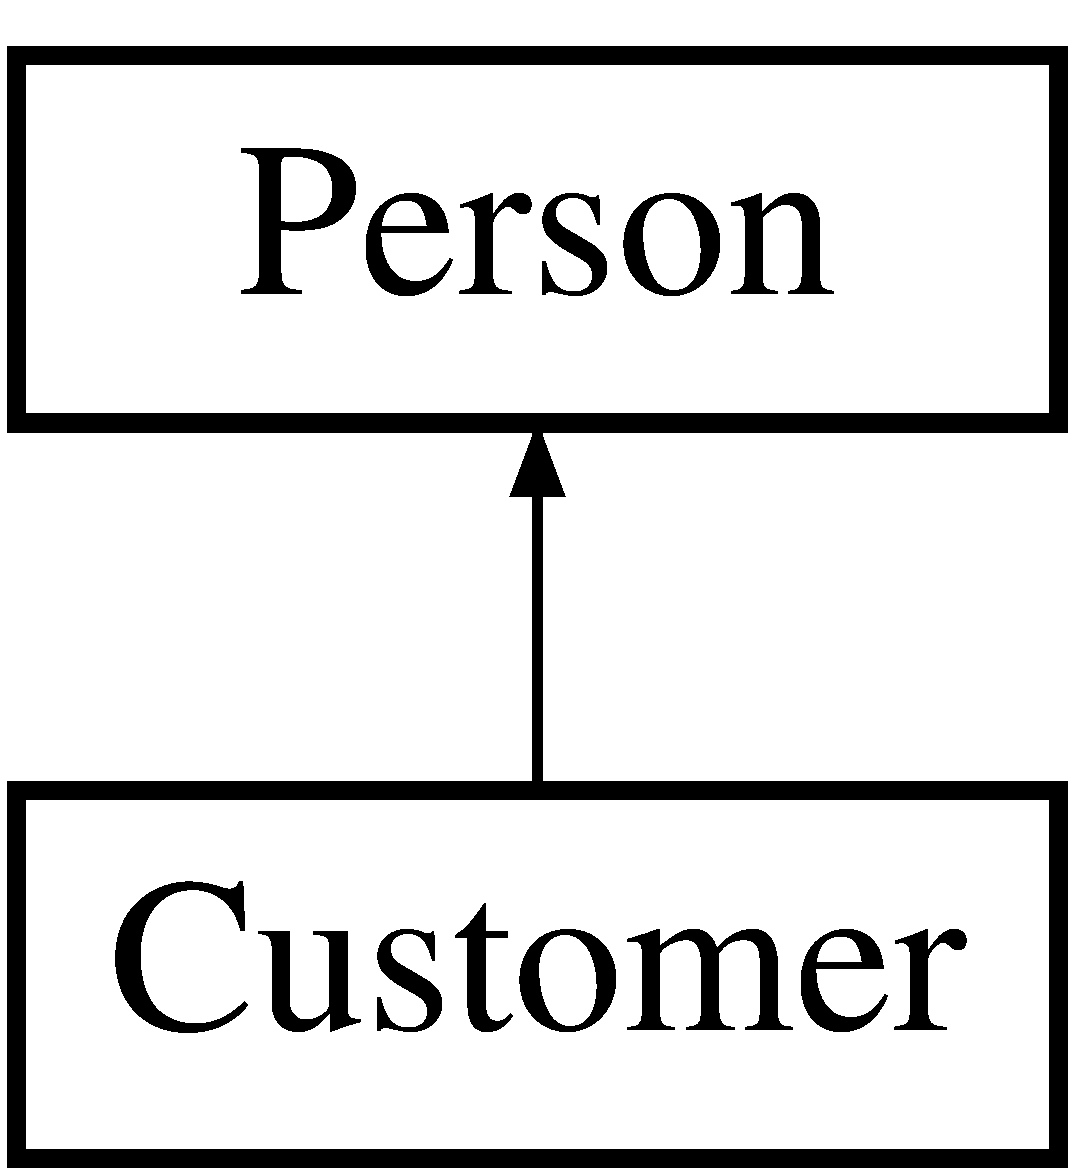
\includegraphics[height=2.000000cm]{class_customer}
\end{center}
\end{figure}
\subsection*{Additional Inherited Members}


The documentation for this class was generated from the following files\+:\begin{DoxyCompactItemize}
\item 
Customer.\+h\item 
Customer.\+cpp\end{DoxyCompactItemize}

\hypertarget{class_employee}{}\section{Employee Class Reference}
\label{class_employee}\index{Employee@{Employee}}
Inheritance diagram for Employee\+:\begin{figure}[H]
\begin{center}
\leavevmode
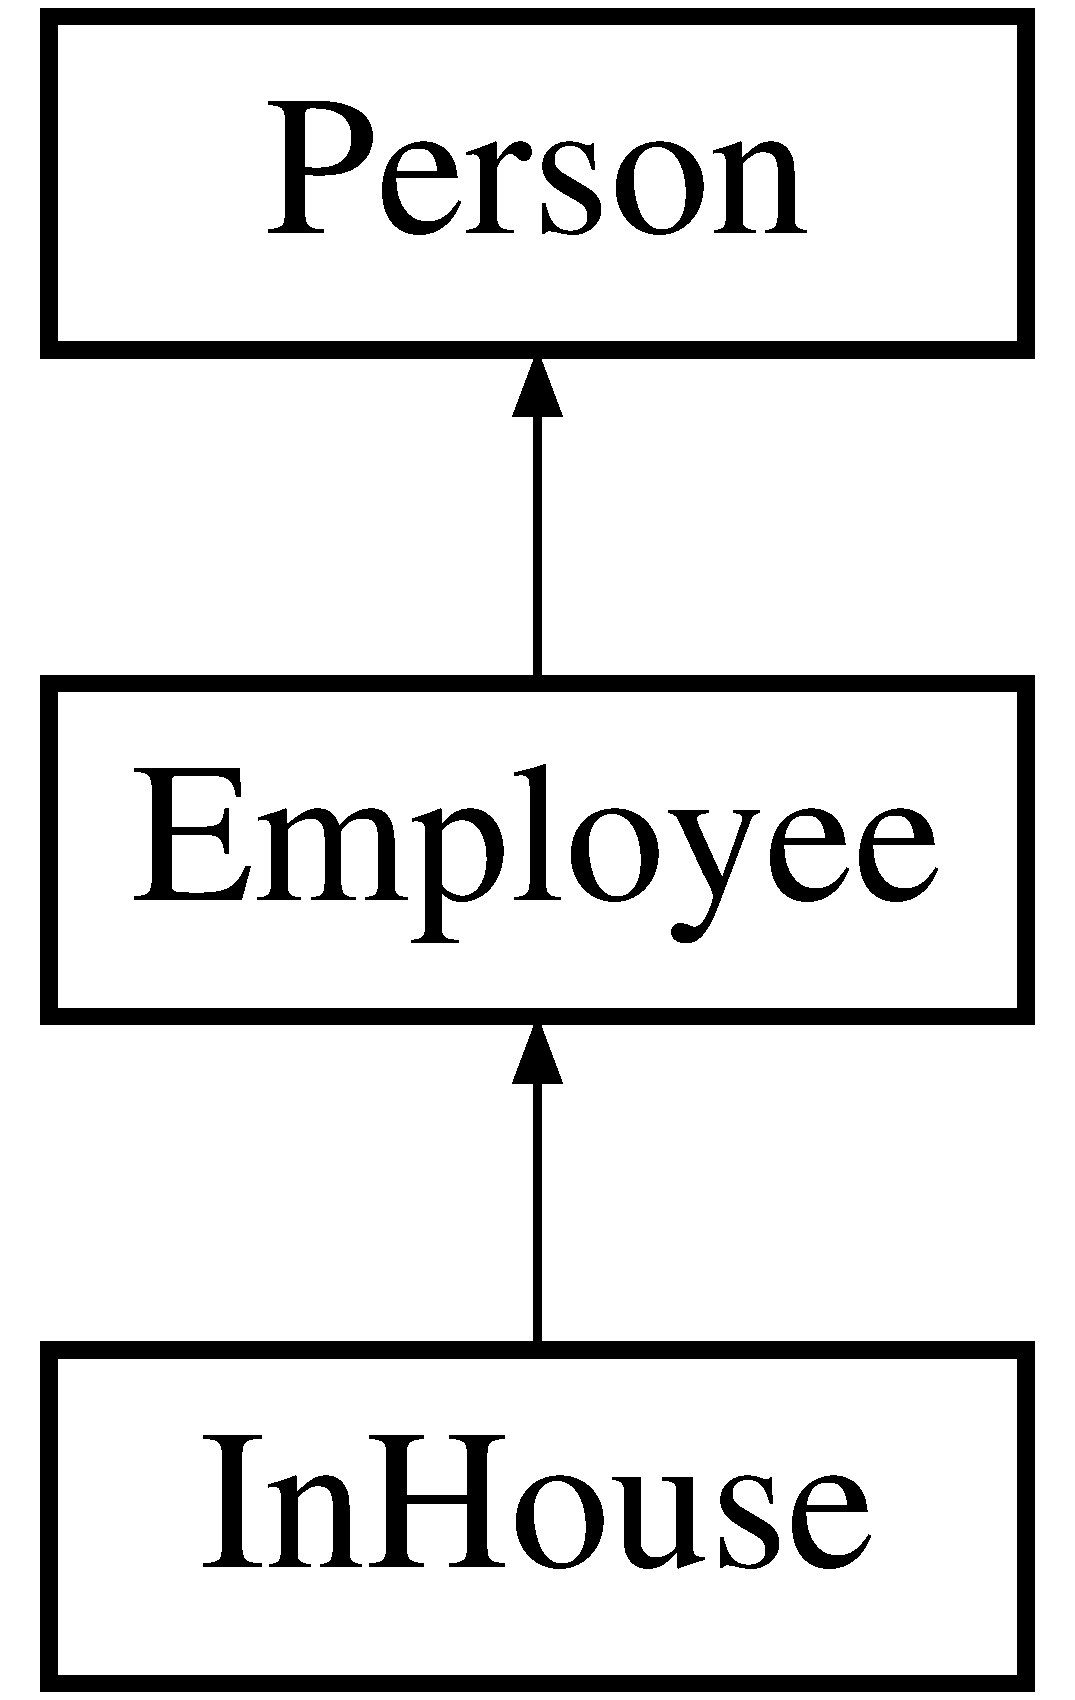
\includegraphics[height=3.000000cm]{class_employee}
\end{center}
\end{figure}
\subsection*{Additional Inherited Members}


The documentation for this class was generated from the following files\+:\begin{DoxyCompactItemize}
\item 
Employee.\+h\item 
Employee.\+cpp\end{DoxyCompactItemize}

\hypertarget{class_in_house}{}\section{In\+House Class Reference}
\label{class_in_house}\index{In\+House@{In\+House}}
Inheritance diagram for In\+House\+:\begin{figure}[H]
\begin{center}
\leavevmode
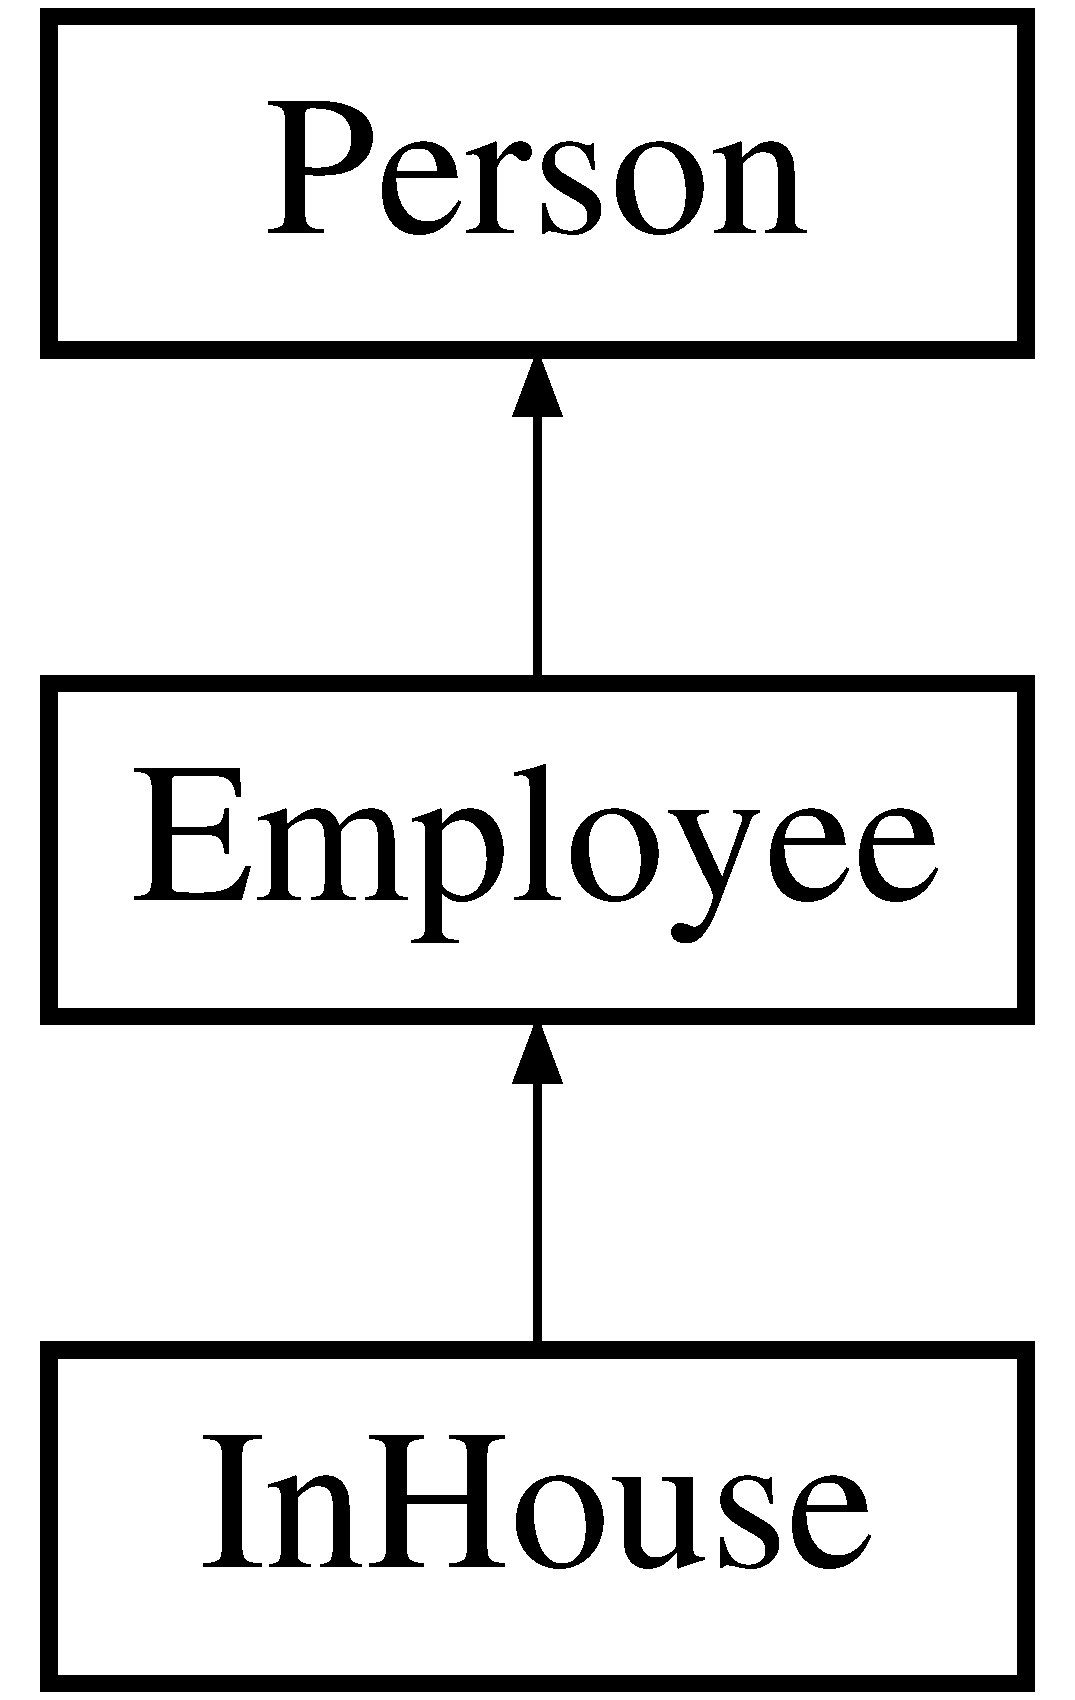
\includegraphics[height=3.000000cm]{class_in_house}
\end{center}
\end{figure}
\subsection*{Additional Inherited Members}


The documentation for this class was generated from the following files\+:\begin{DoxyCompactItemize}
\item 
In\+House.\+h\item 
In\+House.\+cpp\end{DoxyCompactItemize}

\hypertarget{class_linked_list}{}\section{Linked\+List$<$ T $>$ Class Template Reference}
\label{class_linked_list}\index{Linked\+List$<$ T $>$@{Linked\+List$<$ T $>$}}


templated linked list class.  




{\ttfamily \#include $<$Linked\+List.\+h$>$}

\subsection*{Public Member Functions}
\begin{DoxyCompactItemize}
\item 
\mbox{\Hypertarget{class_linked_list_a6b2bd644e74fd8e47598b48dcefe77f9}\label{class_linked_list_a6b2bd644e74fd8e47598b48dcefe77f9}} 
\mbox{\hyperlink{class_linked_list_element}{Linked\+List\+Element}}$<$ T $>$ $\ast$ {\bfseries get\+First} ()
\item 
\mbox{\Hypertarget{class_linked_list_a13d8b4aae07e67358f99486469a5372f}\label{class_linked_list_a13d8b4aae07e67358f99486469a5372f}} 
\mbox{\hyperlink{class_linked_list_element}{Linked\+List\+Element}}$<$ T $>$ $\ast$ {\bfseries get\+Last} ()
\item 
\mbox{\Hypertarget{class_linked_list_a76c1cd46782c1f82064dc79dc69e4f80}\label{class_linked_list_a76c1cd46782c1f82064dc79dc69e4f80}} 
void {\bfseries set\+First} (\mbox{\hyperlink{class_linked_list_element}{Linked\+List\+Element}}$<$ T $>$ $\ast$first)
\item 
\mbox{\Hypertarget{class_linked_list_ace865384dcd68eec6518e1b3d517da3a}\label{class_linked_list_ace865384dcd68eec6518e1b3d517da3a}} 
void {\bfseries set\+Last} (\mbox{\hyperlink{class_linked_list_element}{Linked\+List\+Element}}$<$ T $>$ $\ast$last)
\item 
\mbox{\Hypertarget{class_linked_list_a3f64e4df133e336a6c3b0a705051ad44}\label{class_linked_list_a3f64e4df133e336a6c3b0a705051ad44}} 
void {\bfseries add} (T content)
\item 
\mbox{\Hypertarget{class_linked_list_a075f6a451dcf1df3ff8d00de07195cbd}\label{class_linked_list_a075f6a451dcf1df3ff8d00de07195cbd}} 
void {\bfseries remove} (T content)
\item 
\mbox{\Hypertarget{class_linked_list_af9021d7ddb129042be3b581a16589e1c}\label{class_linked_list_af9021d7ddb129042be3b581a16589e1c}} 
void {\bfseries destroy} ()
\item 
\mbox{\Hypertarget{class_linked_list_ab43bd594a0f7f9ff21c96370da575693}\label{class_linked_list_ab43bd594a0f7f9ff21c96370da575693}} 
void {\bfseries display} ()
\end{DoxyCompactItemize}


\subsection{Detailed Description}
\subsubsection*{template$<$typename T$>$\newline
class Linked\+List$<$ T $>$}

templated linked list class. 

usage\+: Linked\+List$<$your class$>$; 

The documentation for this class was generated from the following file\+:\begin{DoxyCompactItemize}
\item 
Linked\+List.\+h\end{DoxyCompactItemize}

\hypertarget{class_linked_list_element}{}\section{Linked\+List\+Element$<$ T $>$ Class Template Reference}
\label{class_linked_list_element}\index{Linked\+List\+Element$<$ T $>$@{Linked\+List\+Element$<$ T $>$}}
\subsection*{Public Member Functions}
\begin{DoxyCompactItemize}
\item 
\mbox{\Hypertarget{class_linked_list_element_aec3efdfe4e7a3b5798fcc5001be04852}\label{class_linked_list_element_aec3efdfe4e7a3b5798fcc5001be04852}} 
T $\ast$ {\bfseries get\+Content} ()
\item 
\mbox{\Hypertarget{class_linked_list_element_a47f626833cf17b673c3391324c105aba}\label{class_linked_list_element_a47f626833cf17b673c3391324c105aba}} 
\mbox{\hyperlink{class_linked_list_element}{Linked\+List\+Element}}$<$ T $>$ $\ast$ {\bfseries get\+Next} ()
\item 
\mbox{\Hypertarget{class_linked_list_element_a228977625e94b5ff384cbeaab3c1679e}\label{class_linked_list_element_a228977625e94b5ff384cbeaab3c1679e}} 
\mbox{\hyperlink{class_linked_list_element}{Linked\+List\+Element}}$<$ T $>$ $\ast$ {\bfseries get\+Previous} ()
\item 
\mbox{\Hypertarget{class_linked_list_element_acb8b00e8856bf7b034e22d819a7f0967}\label{class_linked_list_element_acb8b00e8856bf7b034e22d819a7f0967}} 
{\bfseries Linked\+List\+Element} (T content, \mbox{\hyperlink{class_linked_list_element}{Linked\+List\+Element}}$<$ T $>$ $\ast$next, \mbox{\hyperlink{class_linked_list_element}{Linked\+List\+Element}}$<$ T $>$ $\ast$previous)
\item 
\mbox{\Hypertarget{class_linked_list_element_a12e8ffd568a87ef6198bdd72c8ce54a1}\label{class_linked_list_element_a12e8ffd568a87ef6198bdd72c8ce54a1}} 
void {\bfseries set\+Content} (T $\ast$content)
\item 
\mbox{\Hypertarget{class_linked_list_element_a43244c7b6686e5719fc1618046d10eb7}\label{class_linked_list_element_a43244c7b6686e5719fc1618046d10eb7}} 
void {\bfseries set\+Next} (\mbox{\hyperlink{class_linked_list_element}{Linked\+List\+Element}}$<$ T $>$ $\ast$next)
\item 
\mbox{\Hypertarget{class_linked_list_element_aaecf5c1df741b1de45448c46ace719b7}\label{class_linked_list_element_aaecf5c1df741b1de45448c46ace719b7}} 
void {\bfseries set\+Previous} (\mbox{\hyperlink{class_linked_list_element}{Linked\+List\+Element}}$<$ T $>$ $\ast$previous)
\item 
\mbox{\Hypertarget{class_linked_list_element_a64d9fa8a99df18fe29619431e3e68da2}\label{class_linked_list_element_a64d9fa8a99df18fe29619431e3e68da2}} 
\mbox{\hyperlink{class_linked_list_element}{Linked\+List\+Element}}$<$ T $>$ $\ast$ {\bfseries insert} (T content)
\item 
\mbox{\Hypertarget{class_linked_list_element_abad575d24768cff94a414901f9b5de69}\label{class_linked_list_element_abad575d24768cff94a414901f9b5de69}} 
void {\bfseries delete\+Element} ()
\end{DoxyCompactItemize}


The documentation for this class was generated from the following files\+:\begin{DoxyCompactItemize}
\item 
Linked\+List\+Element.\+h\item 
Linked\+List\+Element.\+cpp\end{DoxyCompactItemize}

\hypertarget{class_person}{}\section{Person Class Reference}
\label{class_person}\index{Person@{Person}}
Inheritance diagram for Person\+:\begin{figure}[H]
\begin{center}
\leavevmode
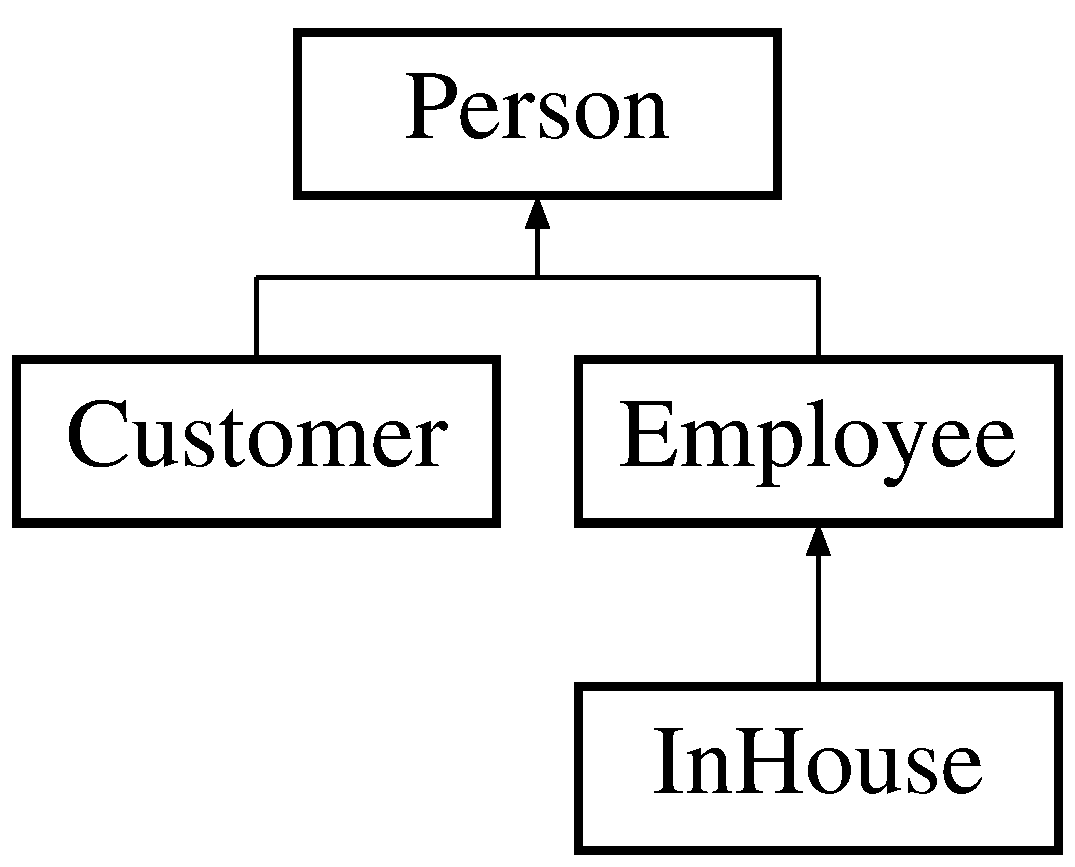
\includegraphics[height=3.000000cm]{class_person}
\end{center}
\end{figure}
\subsection*{Public Member Functions}
\begin{DoxyCompactItemize}
\item 
\mbox{\Hypertarget{class_person_acbc096c55092573ff4abcc2b2b641d04}\label{class_person_acbc096c55092573ff4abcc2b2b641d04}} 
{\bfseries Person} (const char $\ast$first\+\_\+name, const char $\ast$last\+\_\+name, int year)
\item 
\mbox{\Hypertarget{class_person_ab1ac927894f248bdc88f3b65642d7a1b}\label{class_person_ab1ac927894f248bdc88f3b65642d7a1b}} 
{\bfseries Person} (\mbox{\hyperlink{class_person}{Person}} \&person)
\item 
\mbox{\Hypertarget{class_person_aa5bbd58328d2fc888e10e5da888fcd27}\label{class_person_aa5bbd58328d2fc888e10e5da888fcd27}} 
\mbox{\hyperlink{class_person}{Person}} \& {\bfseries operator=} (\mbox{\hyperlink{class_person}{Person}} \&person)
\item 
\mbox{\Hypertarget{class_person_a34adff5582df6e25ab432171a5ac0b88}\label{class_person_a34adff5582df6e25ab432171a5ac0b88}} 
{\bfseries Person} (\mbox{\hyperlink{class_person}{Person}} \&\&)=delete
\item 
\mbox{\Hypertarget{class_person_a46e67bdc77c2ec5c45659c8ab3d1dfbe}\label{class_person_a46e67bdc77c2ec5c45659c8ab3d1dfbe}} 
\mbox{\hyperlink{class_person}{Person}} \& {\bfseries operator=} (\mbox{\hyperlink{class_person}{Person}} \&\&)=delete
\item 
\mbox{\Hypertarget{class_person_aac8ec645eb778c26dd9a9b36946c0a86}\label{class_person_aac8ec645eb778c26dd9a9b36946c0a86}} 
bool {\bfseries set\+First\+Name} (const char $\ast$first\+\_\+name)
\item 
\mbox{\Hypertarget{class_person_ae17d9c12fa0243ff8cf92ec7b5e9edd8}\label{class_person_ae17d9c12fa0243ff8cf92ec7b5e9edd8}} 
bool {\bfseries set\+Last\+Name} (const char $\ast$last\+\_\+name)
\item 
\mbox{\Hypertarget{class_person_a24b9323743af7870100d4d6b2a096be7}\label{class_person_a24b9323743af7870100d4d6b2a096be7}} 
bool {\bfseries set\+Year\+Of\+Birth} (const int year)
\item 
\mbox{\Hypertarget{class_person_a5d95a38a24b0db2695df8de4874a4a16}\label{class_person_a5d95a38a24b0db2695df8de4874a4a16}} 
bool {\bfseries display} ()
\item 
\mbox{\Hypertarget{class_person_a2495b3477c4e48421a3a4ba6099ef92c}\label{class_person_a2495b3477c4e48421a3a4ba6099ef92c}} 
char $\ast$ {\bfseries get\+First\+Name} ()
\item 
\mbox{\Hypertarget{class_person_a253642c10b66ee4d05c8b3669207da0c}\label{class_person_a253642c10b66ee4d05c8b3669207da0c}} 
char $\ast$ {\bfseries get\+Last\+Name} ()
\item 
\mbox{\Hypertarget{class_person_adbff6885ccde40a0bbc23c571fac62e5}\label{class_person_adbff6885ccde40a0bbc23c571fac62e5}} 
int {\bfseries get\+Year\+Of\+Birth} ()
\item 
\mbox{\Hypertarget{class_person_ab383ba032f65b352900e7c182e6d1df9}\label{class_person_ab383ba032f65b352900e7c182e6d1df9}} 
int {\bfseries get\+Count} ()
\item 
\mbox{\Hypertarget{class_person_a49846f9c69c2622dc785c72dd999e673}\label{class_person_a49846f9c69c2622dc785c72dd999e673}} 
int {\bfseries raise\+Count} ()
\end{DoxyCompactItemize}


The documentation for this class was generated from the following files\+:\begin{DoxyCompactItemize}
\item 
Person.\+h\item 
Person.\+cpp\end{DoxyCompactItemize}

%--- End generated contents ---

% Index
\backmatter
\newpage
\phantomsection
\clearemptydoublepage
\addcontentsline{toc}{chapter}{Index}
\printindex

\end{document}
